\documentclass[serif,xcolor=pdftex,dvipsnames,table,hyperref={bookmarks=false,breaklinks}]{beamer}

%%%%%%%%%%%%%%%%
% Change the macros below to configure the title slides
% for your course.
\newcommand{\coursename}{COMPSCI 589}
\newcommand{\instructor}{Benjamin M. Marlin}
\newcommand{\university}{University of Massachusetts Amherst}
\newcommand{\department}{College of Information and Computer Sciences}
%%%%%%%%%%%%%%%%


\newcommand{\settitlecard}[2]{
  \title[\coursename  Lecture #1] 
    {\coursename \\ Lecture #1: #2}
     \author[\instructor]{\instructor}
     \institute[\university]{
     \department\\
     \university
   }
\date{}
}

\newcommand{\maketitlepage}{
  \begin{frame}
  \titlepage
  \center{
    %If you use the slides unmodified, retain the attribution below
    \tiny{Slides by Benjamin M. Marlin (marlin@cs.umass.edu). \\
    \vspace{-1em}Created with support from National Science Foundation Award\# IIS-1350522. 
    %If you modify the slides, please retain the alternate attribution below
    %\tiny{Based on slides by Benjamin M. Marlin (marlin@cs.umass.edu). \\    
    %\vspace{-1em}Created with support from National Science Foundation Award\# IIS-1350522. 
    }                                              
  }  
  \end{frame}
}

\AtBeginSection[]
{
  \begin{frame}<beamer>{Outline}
    \tableofcontents[currentsection,subsectionstyle=hide]
  \end{frame}
}


\newcommand{\cut}[1]{}

\newcommand{\iconbox}[4]{
  \only<#1-#2>{
    \begin{columns}[T]
      \column{0.5in}
           \includegraphics[width=0.5in]{#3}
       \column{3.7in}
            #4
    \end{columns}
    \medskip
    \medskip
    \medskip
  }
}

\mode<presentation>{
  \usepackage{../beamertheme589theme}
  \setbeamercovered{invisible}
}

\mode<handout>{
  \usepackage{../beamertheme589theme}
  \setbeamercovered{transparent}
}


\usepackage[english]{babel}
\usepackage[latin1]{inputenc}
\usepackage{times}
\usepackage[T1]{fontenc}
\usepackage{amsmath}
\usepackage{amssymb}
\usepackage[noend]{algorithmic}
\usepackage{algorithm}
\usepackage{listings}

\renewcommand\mathfamilydefault{\rmdefault}

\newcommand{\setA}{\mathcal{A}}
\newcommand{\setB}{\mathcal{B}}
\newcommand{\setS}{\mathcal{S}}
\newcommand{\setV}{\mathcal{V}}
\DeclareMathOperator*{\union}{\bigcup}
\DeclareMathOperator*{\intersection}{\bigcap}
\DeclareMathOperator*{\Val}{Val}
\newcommand{\mbf}[1]{{\mathbf{#1}}}
\DeclareMathOperator*{\argmax}{arg\,max}
\DeclareMathOperator*{\argmin}{arg\,min}
\DeclareMathOperator*{\sign}{sign}
\newcommand{\deriv}[2]{\frac{\partial{#1}}{\partial{#2}}}


\settitlecard{21}{Kernel Principal Components \\Analysis and Spectral Clustering}

\begin{document}

\maketitlepage


\section{Kernel PCA}
\subsection{Foo}

\begin{frame}[t]{Limitations of LDR}

\begin{itemize}
\item All the dimensionality reduction methods we've seen so far find optimal
linear sub-spaces under different constraints.

\pause\item \textbf{Question:} How can we move beyond linear sub-spaces?
\end{itemize} 
\end{frame}

\begin{frame}[t]{Basis Expansion}

\begin{itemize}
\item One way to move beyond linear dimensionality reduction is to first apply 
a non-linear basis expansion to the data vectors, and then apply linear 
dimensionality reduction.
 
\pause\item Any basis expansion can be applied including polynomials, etc., 
just as in the case of classification and regression.
 
\end{itemize} 
\end{frame}

\begin{frame}[t]{Basis Expansion + SVD}

Given a data set $\mbf{X}\in\mathbb{R}^{N\times D}$ and a basis expansion 
function $\phi: \mathbb{R}^D \rightarrow \mathbb{R}^{D'}$ for $D'>D$, we obtain 
the following SVD-based algorithm:

\begin{enumerate}
 \pause \item Compute $\mbf{U},\mbf{S},\mbf{V} = \mbox{SVD}(\phi(\mbf{X}))$
 \pause \item Return $Z = \mbf{U}\mbf{S}$
\end{enumerate} 
\end{frame}

\begin{frame}[t]{Basis Expansion + PCA}

Given a data set $\mbf{X}\in\mathbb{R}^{N\times D}$ and a basis expansion 
function $\phi: \mathbb{R}^D \rightarrow \mathbb{R}^{D'}$ for $D'>D$, we obtain 
the following PCA-based algorithm:

\begin{enumerate}
\pause \item Compute $\Sigma = (\phi(\mbf{X})-\mu)^T(\phi(\mbf{X})-\mu)$ where 
$\mu=1/N\sum \phi(\mbf{X}_i)$.

\pause\item Compute the $K$ leading eigenvectors $w_1,...,w_K$ of $\Sigma$ 
where $\mbf{w}_k \in \mathbb{R}^{D'}$.

\pause\item Stack the eigenvectors together into a $D' \times K$ matrix 
$\mbf{W}$ where each column $k$ of $\mbf{W}$ corresponds to $\mbf{w}_k$.

\pause\item Project the matrix $\phi(\mbf{X})$ into the rank-K sub-space of 
maximum variance by computing the matrix product $\mbf{Z}=\phi(\mbf{X})\mbf{W}$.
\end{enumerate} 
\end{frame}

\begin{frame}[t]{Kernel PCA}
\begin{itemize}
\item As in the classification case, it becomes very expensive to use an 
explicit basis function expansion that maps data into a high-dimensional space.

\pause\item In the basic SVD-based algorithm, there's no way to avoid this 
problem.

\pause\item In the PCA-based algorithm, it's not hard to show that the sample 
covariance matrix obtained after the basis expansion depends only on inner 
products of the form $\langle\phi(\mbf{X}_i),\phi(\mbf{X}_j)\rangle$. 

\pause\item Kernel functions can often provide a much more efficient 
computation of these inner products without explicitly computing the basis 
expansion: $\mathcal{K}(\mbf{X}_i, \mbf{X}_j) = 
\langle\phi(\mbf{X}_i),\phi(\mbf{X}_j)\rangle$
\end{itemize}
\end{frame}

\begin{frame}[t]{Kernel PCA Algorithm}
Given a data set $\mbf{X}\in\mathbb{R}^{N\times D}$ and a kernel function 
$\mathcal{K}$, Kernel PCA can be computed as follows:

\begin{enumerate}
\pause\item Compute $\mathbf{K}_{ij} = \mathcal{K}(\mbf{X}_i,\mbf{X}_j)$ for 
all $i,j$

\pause\item Compute $\Sigma = (I-1_N)\mathbf{K}(I-1_N)$ where $1_N$ is an $NxN$ 
matrix where every entry is $1/N$.

\pause\item Compute the $K$ leading eigenvectors $w_1,...,w_K$ of $\Sigma$ 
where $\mbf{w}_k \in \mathbb{R}^N$ along with their eigenvalues 
$\lambda_1,...,\lambda_K$

\pause\item Compute the elements of the matrix of projected data vectors using
$$\mbf{Z}_{nk} = \sum_{i=1}^N \frac{\mbf{w}_{ik}}{\lambda_k} 
\mathcal{K}(\mbf{X}_n,\mbf{X}_i)$$
\end{enumerate} 
\end{frame}

\begin{frame}[t]{Example}

Consider the case of using the radial basis function kernel
$\mathcal{K}(\mbf{x},\mbf{y}) = \exp(-\frac{1}{c}||\mbf{x}-\mbf{y}||_2^2)$.

\center
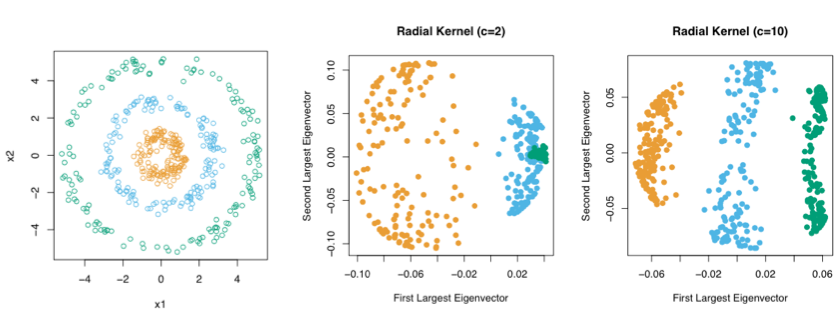
\includegraphics[width=4in]{../Figures/kpca.png}

\end{frame}

\begin{frame}[t]{Summary}

\begin{itemize}
\item Kernel PCA provides a non-linear dimensionality reduction method that can 
be used to extract directions of variation after applying high-dimensional 
basis function expansions, without explicitly performing the basis expansion.

\pause\item Kernel PCA can be thought of as looking for directions of variation 
in the space of similarities between data cases, and can extract components 
that correspond to fairly complex structures.

\pause\item When a good kernel is known a priori, kernel PCA can provide an
effective pre-processing step for clustering methods as well as linear 
classification and regression methods.  

\pause\item However, exact computation of kernel PCA can be expensive because 
the size of the matrix that is decomposed is $NxN$.
\end{itemize} 

\end{frame}

\section{Spectral Clustering}
\subsection{Foo}

\begin{frame}[t]{Spectra Clustering}

\begin{itemize}
\item Applying kernel PCA followed by K-means clustering is closely related to 
a clustering method called spectral clustering.

\pause\item Spectral clustering works by defining a weighted 
similarity graph on the data cases. 

\pause\item It's very common to use $\mathcal{K}(\mbf{x},\mbf{y}) = 
\exp(-\frac{1}{c}||\mbf{x}-\mbf{y}||_2^2)$ as the weighting function and to 
include edges corresponding to the $K$ nearest neighbors of each point.

\pause\item Unlike the kernel PCA case, the similarity values for
edges not included in the graph are set to $0$. The matrix of edge weights is 
denoted by $\mathbf{W}$.

\end{itemize} 

\end{frame}


\begin{frame}[t]{Connected Components}

\begin{itemize}
\item In the simple case, the resulting graph has multiple connected 
components, and we can create one cluster for each connected component.

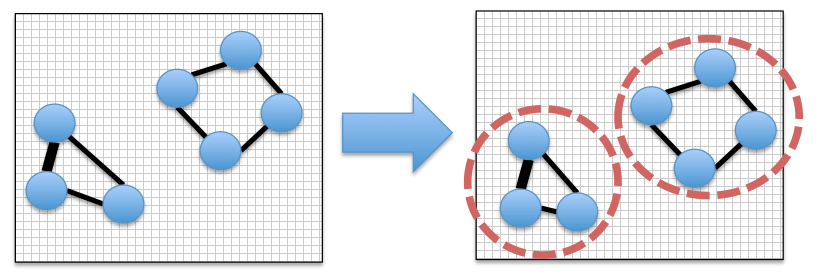
\includegraphics[width=4in]{../Figures/spectral_clustering1.png}

\end{itemize} 

\end{frame}

\begin{frame}[t]{Minimum Weight Balanced Cut}

\begin{itemize}
\item In the more complex case, the graph has only one connected component, and
the goal is to identify a minimum weight balanced cut:

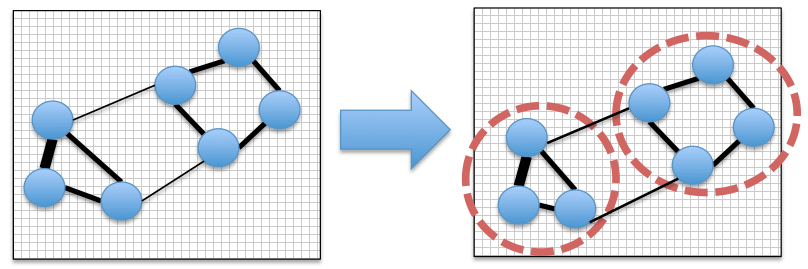
\includegraphics[width=4in]{../Figures/spectral_clustering2.png}

\end{itemize} 

\end{frame}


\begin{frame}[t]{Spectral Clustering Algorithm}

\begin{itemize}
\item Define the weighted node degree matrix $\mbf{D}$ such that $\mbf{D}_{ii} 
= \sum_n \mathbf{W}_{in}$.

\pause\item Define the graph laplacian $\mbf{L} = \mbf{D} - \mbf{W}$.

\pause\item Compute the eigendecomposition of $\mathbf{L}$ and extract the 
$M$ eigenvectors corresponding to the $M$ smallest eigenvalues. 

\pause\item Just like in kernel PCA, each eigenvector is length $N$. The 
collection of $M$ of them forms an alternative dimensionality reduced 
representation for $\mbf{X}$, which we can call $\mbf{Z}$.

\pause\item Run K-means on $\mbf{Z}$ to extract $K$ clusters.

\pause\item This algorithm is an approximation to the exact $K$-way min-cut in 
the graph, which has exponential complexity to compute. 

\end{itemize} 

\end{frame}





\end{document}
